\section{Pruebas y Resultados}

Para poner a prueba nuestras implementaciones, lo que haremos en principio, será probar con casos pequeños, donde esperamos tener resultados previsibles. Luego iremos aumentando la cantidad de páginas y veremos la performance de la implementación.

\subsection{Testeando con Casos Pequeños}

Veamos algunos casos chicos:

\begin{itemize}
    \item \textbf{Caso con 4 páginas} En este caso tenemos 4 páginas relacionadas de esta manera:
        \begin{enumerate}
            \item $a \leadsto b$
            \item $a \leadsto c$
            \item $a \leadsto d$
            \item $b \leadsto c$
            \item $b \leadsto d$
        \end{enumerate}

        Como vemos tenemos $c$ y $d$ como las páginas mas referenciadas, por lo cual es de esperar pensar que el resultado tiene que dar que estos son los que tienen mayor ranking. Veamos pues el resultado luego de aplicar el método directo:

        \begin{itemize}
            \item $a = 0.168327$
            \item $b = 0.216019$
            \item $c = 0.307827$
            \item $d = 0.307827$
        \end{itemize}

        Ahora veamos los resultados con el método iterativo, con 10 iteraciones y $k = 0.001$:

        \begin{itemize}
            \item $a = 0.168327$
            \item $b = 0.216019$
            \item $c = 0.307827$
            \item $d = 0.307827$
        \end{itemize}

        Tambíén con 1000 iteraciones terminó dando lo mismo.

        \item \textbf{Caso con 7 páginas}

	Aca tenemos un conjunto de 7 páginas y 18 links, relacionadas como vemos en el gráfico:
        \newpage
            \begin{figure}
                \centering
                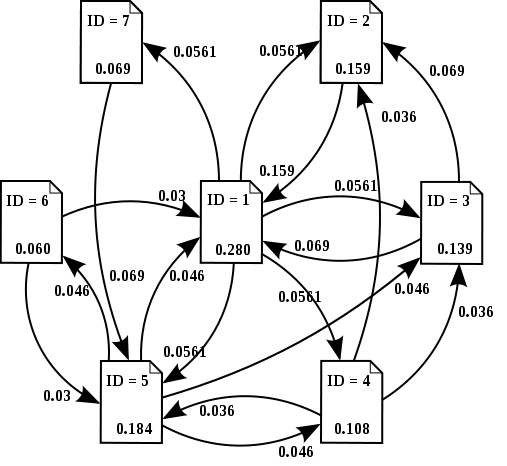
\includegraphics[scale=0.60]{../graficos/507px-Linkstruct3.png}
                % 507px-Linkstruct3.svg.png: 507x466 pixel, 72dpi, 17.89x16.44 cm, bb=0 0 507 466
                \label{fig: Caso con 7 Páginas}
            \end{figure}

        Como bien se ve en el gráfico esperamos que la página de ID = 1, sea la que tenga mayor ranking. Aplicamos el método directo y nos quedó:

        \begin{itemize}
          \item \textbf{ID 1} $= 0.280288$
          \item \textbf{ID 2} $= 0.158764$
          \item \textbf{ID 3} $= 0.138882$
          \item \textbf{ID 4} $= 0.10822$
          \item \textbf{ID 5} $= 0.184198$
          \item \textbf{ID 6} $= 0.0605707$
          \item \textbf{ID 7} $= 0.0690775$
        \end{itemize}

        Luego aplicamos el iterativo, con 10 iteraciones y residuo $0.001$:

        \begin{itemize}
          \item \textbf{ID 1} $= 0.274751$
          \item \textbf{ID 2} $= 0.157001$
          \item \textbf{ID 3} $= 0.138479$
          \item \textbf{ID 4} $= 0.108889$
          \item \textbf{ID 5} $= 0.18545$
          \item \textbf{ID 6} $= 0.0643551$
          \item \textbf{ID 7} $= 0.0710757$
        \end{itemize}	

        Ahora con 100 iteraciones, mismo residuo:

        \begin{itemize}
          \item \textbf{ID 1} $= 0.280281$
          \item \textbf{ID 2} $= 0.158762$
          \item \textbf{ID 3} $= 0.138881$
          \item \textbf{ID 4} $= 0.10822$
          \item \textbf{ID 5} $= 0.1842$
          \item \textbf{ID 6} $= 0.0605753$
          \item \textbf{ID 7} $= 0.0690799$
        \end{itemize}	

        Con 1000 iteraciones nos quedó el mismo resultado.

	\item \textbf{Caso con 11 páginas}
	Aquí tenemos 11 páginas y un total 17 links, en el gráfico ilustrada, aparecen sus relaciones:

	\begin{center}
	  \centering
	  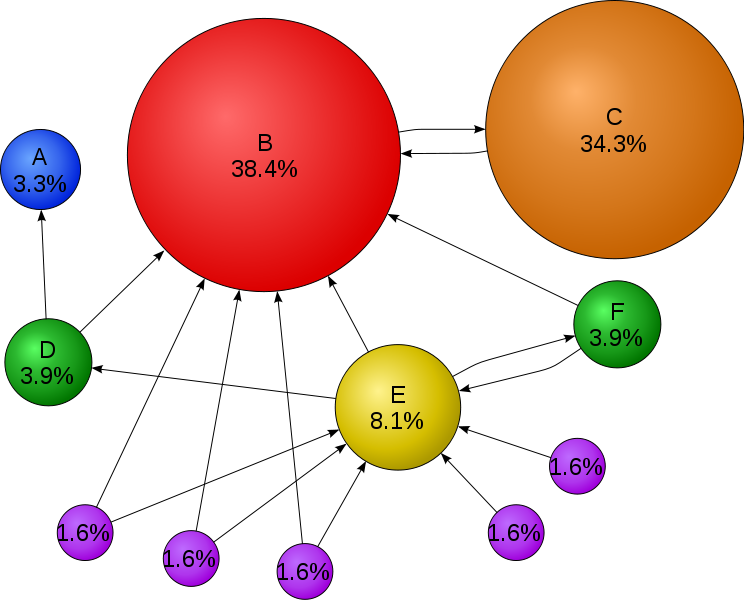
\includegraphics[scale=0.4]{../graficos/744px-PageRanks-Example.png}
	  % 744px-PageRanks-Example.svg.png: 744x600 pixel, 72dpi, 26.25x21.17 cm, bb=0 0 744 600
	  \label{fig: Caso con 11 páginas}
	\end{center}

        Acá esperamos que las páginas B y C, sean las que mas ranking tengan y seguida por la E. Aplicando el directo:

        \begin{itemize}
            \item $A = 0.0327815$
            \item $B = 0.384401$
            \item $C = 0.34291$
            \item $D = 0.0390871$
            \item $E = 0.0808857$
            \item $F = 0.0390871$
            \item $G = 0.0161695$
            \item $H = 0.0161695$
            \item $I = 0.0161695$
            \item $J = 0.0161695$
            \item $K = 0.0161695$
        \end{itemize}

        Luego el iterativo con 10 iteraciones y residuo $0.001$:

        \begin{itemize}
            \item $A = 0.0399942$
            \item $B = 0.361587$
            \item $C = 0.30572$
            \item $D = 0.0476854$
            \item $E = 0.0986861$
            \item $F = 0.0476854$
            \item $G = 0.0197284$
            \item $H = 0.0197284$
            \item $I = 0.0197284$
            \item $J = 0.0197284$
            \item $K = 0.0197284$
        \end{itemize}

        Con 100 iteraciones mismo residuo:
        \begin{itemize}
            \item $A = 0.0327861$
            \item $B = 0.384386$
            \item $C = 0.342886$
            \item $D = 0.0390926$
            \item $E = 0.0808971$
            \item $F = 0.0390926$
            \item $G = 0.0161718$
            \item $H = 0.0161718$
            \item $I = 0.0161718$
            \item $J = 0.0161718$
            \item $K = 0.0161718$
        \end{itemize}

        Con 1000 iteraciones, quedaron los mismos resultados.
\end{itemize}

También propusimos un caso de test en el cual todos las paginas estan relacionadas entre sí, es decir un grafo completo. Como era de esperarse tanto para el iterativo como para el directo, el ranking de cada uno de las páginas quedó $0.05$. En esto nuestro cantidad de páginas analizadas fueron 20.

\subsection{Iteraciones vs. Residuo}

A continuación estudiaremos la relacion entre la cantidad de iteraciones y el residuo resultante, este estudio nos permitira evaluar la velocidad de convergencia del método iterativo.

Como caso de estudio, elegimos el caso provisto por la catedra de la wikipedia en Interlingua.

\begin{center}
  \centering
  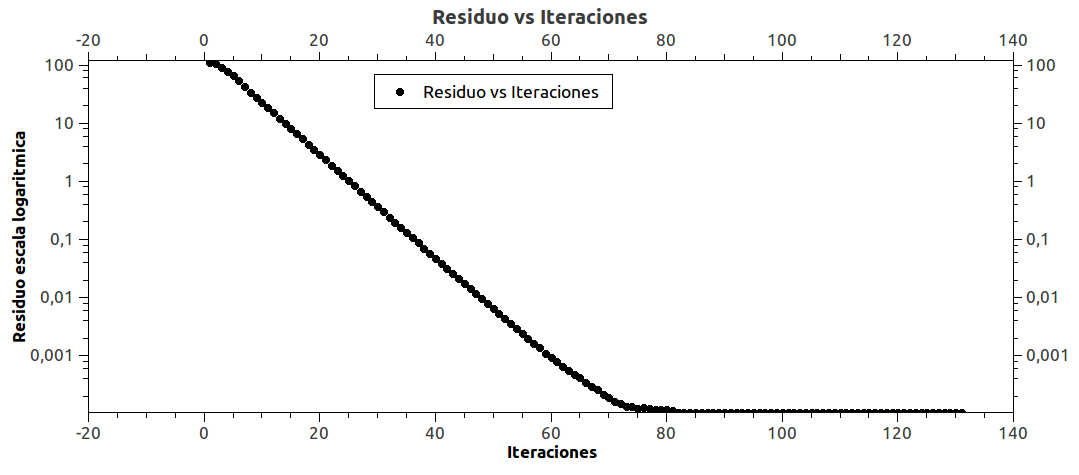
\includegraphics[scale=0.6]{../graficos/residuo_vs_iteraciones.png}
  % 744px-PageRanks-Example.svg.png: 744x600 pixel, 72dpi, 26.25x21.17 cm, bb=0 0 744 600

  \label{fig: Iteraciones vs Residuo}
\end{center}

\subsection{Testeando casos grandes}

Dados los casos de tamaño mediano a grande, nos encontramos con lo siguiente, el método directo tarda un tiempo no razonable, dado el tamaño de los mismos, sin embargo el método iterativo para los casos intermedios se comporta lento, pero de forma aceptable, dando algùn resultado aproximado. 

Vimos que mostrar los resultados de los casos intermedios a grandes, no aporta a la discusiòn, por lo tanto, mostramos que casos de los provistos por la catedra pudieron ejecutar como máximo los diferentes algoritmos.

\begin{itemize}
 \item Directo: Wikidump - Extremeño (2395 páginas, 19084 links)
 \item Directo: Obama transition (páginas 30002, 379871 links)
\end{itemize}

